\documentclass[10pt,a4paper]{article}
\usepackage[utf8]{inputenc}
\usepackage{amsmath}
\usepackage{gensymb}
\usepackage{amsfonts}
\usepackage{siunitx}
\usepackage[european]{circuitikz}
\usepackage{geometry}
\newgeometry{tmargin=2cm, bmargin=2cm, lmargin=2cm, rmargin=2cm}
\usepackage{amssymb}
\usepackage{polski}
\usepackage{graphicx}
\author{\textbf{T. Fąs}}
\title{\textbf{Radon w powietrzu}}
\begin{document}
\maketitle

\begin{center}
\textbf{\subsection*{STRESZCZENIE}}
\end{center}
Celem doświadczenia był pomiar stężenia $^{222}$Ra i produktów jego rozpadu w powietrzu oraz ocena energii cząstek $\alpha$ powstałych w wyniku jego rozpadu. Niestety, na skutek błędów w pomiarach, możliwe było tylko wyznaczenie stężenia $C_{A}$ $^{218}$Po oraz ocena energii $E$ cząstek $\alpha$. Wynoszą one: $C_{A}=0,75\pm0,21$ Bq/m$^3$ i $E\approx 7,14$ MeV.
\begin{center}
\textbf{\subsection*{WSTĘP}}
\end{center}
W otoczeniu człowieka istnieje wiele naturalnych źródeł promieniotwórczych. Jednym z nich jest rozpad $^{238}$U znajdującego się w skorupie ziemskiej, który po czterech rozpadach $\alpha$ i dwóch rozpadach $\beta$ prowadzi do radonu 222. Radon jest gazem szlachetnym, który wydostaje się z gleby, miesza się z powietrzem i przykleja się do aerozoli atmosferycznych. W ten sposób trafia on do mieszkań lub do płuc. Innym źródłem $^{222}$Rn mogą być materiały budowlane, jeśli te zawierają w sobie pierwiastki takie jak rad, uran czy tor. Radon powstaje w wyniku rozpadu tych pierwiastków. 

Łańcuch rozpadu $^{222}$Rn wygląda następująco:
\begin{center}
$^{222}$Rn 
$\xrightarrow{\text{3,8 d, $\alpha$}}$
 $^{218}$Po 
 $\xrightarrow{\text{3,05 min, $\alpha$}}$
  $^{214}$Pb
 $\xrightarrow{\text{26,8 min, $\beta$}}$
  $^{214}$Bi
 $\xrightarrow{\text{19,8 min, $\beta$}}$
  $^{214}$Po,
\end{center}
przy czym na strzałkach podano czasy połowicznego rozpadu danego pierwiastka oraz jego rodzaj. Analiza tych rozpadów metodą Markova pozwoli na wyznaczenie stężenia $^{222}$Rn w powietrzu.

Metoda Markova \cite{m1} polega na pompowaniu powietrza przez filtr, na którym będą odkładać się produkty rozpadu radonu. Następnie dokonuje się dwóch pomiarów liczby cząstek $\alpha$, które emituje ten filtr. Na tej podstawie można wyznaczyć stężenie np. polonu 218. Dla cyklu postaci 5 minut pompowania, minuta przerwy, 3 minuty zliczeń cząstek $\alpha$, 3 minuty przerwy i 3 kolejne minuty zliczeń, aktywność $C_{A}$ polonu można wyznaczyć ze wzoru:
\begin{equation}
C_{A}=\frac{7,3\cdot10^{-5}\left(N_{1}-N_{2}\right)}{\epsilon v \eta},
\end{equation}
gdzie $N_{1}$ i $N_{2}$ to liczba zliczeń uzyskanych kolejno w pierwszym i drugim pomiarze cząstek $\alpha$, $v$ jest prędkością pompowania powietrza w m$^3$/s, $\epsilon$ to wydajność rejestracji cząstek $\alpha$, a $\eta$ to skuteczność filtra w zatrzymywaniu produktów rozpadu radonu. Współczynnik $7,5\cdot10^{-5}$ został wyznaczony dla tego konkretnego cyklu pomiarowego. 
Aby poznać udział innych produktów rozpadu radonu, należy zmierzyć intensywność $I_{\alpha}$ promieniowania $\alpha$ emitowanego przez próbkę. W tym celu należy wykonać serię krótkich pomiarów zliczeń cząstek $\alpha$, aby poznać zależność liczby zliczeń na sekundę od czasu. Zależność ta powinna być zgodna ze wzorem:
\begin{equation}
I_{\alpha}=\epsilon\eta v \left(A \exp(-\lambda_{A}t)+B \exp(-\lambda_{B}t)+C \exp(-\lambda_{C}t) \right),
\end{equation}
gdzie $\lambda_{i}$ jest stałą rozpadu kolejno dla $^{218}$Po (A), $^{214}$Pb (B) i $^{214}$Bi (C). A, B i C to stałe, których związek z aktywnością produktów rozpadu radonu jest następujący:

\begin{equation}
A=184C_{A} 
\end{equation}
\begin{equation}
B=139C_{A}+1084C_{B}
\end{equation}
\begin{equation}
C=-143C_{A} -1060 C_{B} + 275 C_{C}.
\end{equation} 
Pozostałe symbole mają to samo znaczenie, co wyżej.

Wyznaczenie energii cząstki $\alpha$ wiąże się z wyznaczeniem jej maksymalnego zasięgu. W ten sposób, korzystając z gotowych tablic zależności zasięgu od energii, można odczytać energię cząstki.





\begin{center}
\textbf{\subsection*{UKŁAD DOŚWIADCZALNY I SCHEMAT POMIARÓW}}
\end{center}
Przyrządy użyte w doświadczeniu to: scyntylator, fotopowielacz, zasilacz, licznik zliczeń cząstek, odkurzacz, filtr z bawełny, miernik przepływu powietrza oraz taśma miernicza, stoper i podstawka o kontrolowanej wysokości. Scyntylator był przykryty cienką warstwą folii aluminiowej, by blokować dostęp światła do fotopowielacza. Dodatkowo całość byłą chroniona siatką. Odległość od siatki do folii wynosiła około 2 mm. Fotopowielacz podłączony był do licznika. Schemat układu znajduje się na Rysunku 1A. 

\begin{figure}[h!]
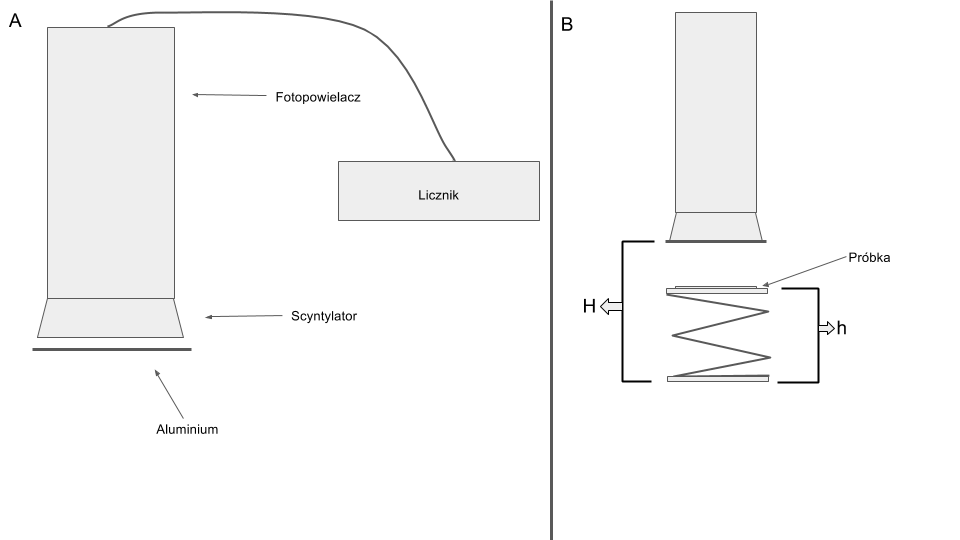
\includegraphics[width=12cm]{radon} 
\centering
\caption{Schemat układu doświadczalnego}
\label{p1}
\end{figure}

Do końcówki odkurzacza zamocowano filtr z bawełny, a do wylotu odkurzacza zamontowano miernik przepływu powietrza. W ten sposób można było jednocześnie zbierać radon jak i zebrać dane pozwalające na pomiar prędkości przepływu powietrza przez odkurzacz. Końcówkę z filtrem umieszczono przy podłodze, w słabo wentylowanym miejscu. Pozwoliło to na zebranie większej próbki. Czas zasysania jak i czas pomiarów mierzono stoperem. Przed włączeniem odkurzacza spisywano stan miernika przepływu, oznaczony jako $V_{1}$. Zgodnie z metodą Markowa powietrze zasysano przez czas $t=5$ minut, po tym czasie zatrzymywano odkurzacz i spisywano stan końcowy miernika $V_{2}$. Różnica tych wartości podzielona przez czas daje prędkość zasysania powietrza w m$^3$/s. Po upływie minuty od wyłączenia odkurzacza filtr z bawełny zostaje umieszczony na detektorze cząstek $\alpha$. Detektor podłączony jest do licznika, który zlicza trafienia z fotopowielacza. Pomiar przeprowadzono zgodnie ze schematem Markova. Przed każdym pomiarem licznik zerowano.

Podobny schemat miał miejsce w trakcie pomiaru intensywności promieniowania, z tą różnicą, że zamiast trzyminutowych pomiarów wykonano wiele kilkunastosekundowych pomiarów. Otrzymane wyniku należało podzielić przez czas zliczanie i powiązać z czasem, który upłyną od rozpoczęcia pomiarów. 

Do wyznaczenia energii cząstek $\alpha$ wykorzystano źródło, które promieniowało silniej niż filtr z wcześniejszych pomiarów. Odległość między źródłem a detektorem wyznaczano w sposób pośredni: odejmowano od stałej wysokości $H$ detektora wysokość $h$ podnośnika (Rysunek 1B). Dla każdej wysokości wykonano po dwa pomiary trwające 10 sekund. 

\begin{center}
\textbf{\subsection*{WYNIKI POMIARÓW}}
\end{center}
Wyniki dla pierwszego z pomiarów przedstawiono w Tabeli 1. Parametry $\eta$ i $\epsilon$ oszacowano. Filtr wykonany był z grubej bawełny, dlatego też założono, że $\eta=1$. Wartość $\epsilon$ oszacowano na 0,4, ponieważ połowa cząstek nie trafi do detektora (poleci w drugą stronę), a część cząstek do niego nie doleci, gdyż zostanie zatrzymana przez powietrze lub siatkę ochronną i aluminium.

\begin{table}[h!]
\centering
\caption{Wyniki pomiarów I}
\label{t1}
\begin{tabular}{|c|c|c|c|c|c|c|}
\hline
Wielkość & $N_{1}$ & $N_{2}$ & $V_{1}$  & $V_{2}$  & $\eta$ & $\epsilon$ \\ \hline
Wartość  & 127   & 70    & 11,488 & 15,632 & 1      & 0,4        \\ \hline
\end{tabular}
\end{table}

Niestety, dane uzyskane dla drugiego pomiaru (pomiar intensywności promieniowania) nie nadają się do analizy, gdyż eksperymentator zamiast wykonania serii krótkich zliczeń powtórzył schemat poprzedniego pomiaru.

Wyniki pomiarów zasięgu cząstek $\alpha$ przedstawiono w Tabeli 2, dla wysokości $H=23$ cm.
\begin{table}[h!]
\centering
\caption{Pomiary odległości i zliczeń.}
\label{t2}
\begin{tabular}{|c|c|c|c|c|c|c|}
\hline
h [cm]     & 18,5 & 18  & 17,5 & 17 & 16,5 & 16 \\ \hline
$n_{1}$ & 226  & 124 & 82   & 63 & 28   & 26 \\ \hline
$n_{2}$ & 235  & 111 & 113  & 67 & 43   & 20 \\ \hline
\end{tabular}
\end{table}


\begin{center}
\textbf{\subsection*{ANALIZA DANYCH}}
\end{center}

W pierwszej kolejności postanowiono zbadać niepewności urządzeń pomiarowych. W przypadku przepływomierza czy taśmy mierniczej podstawowym źródłem niepewności była dokładność urządzenia wynikająca ze skali. W przypadku stopera należało dodatkowo uwzględnić czas reakcji $t_{r}$ obserwatora. Czas ten oszacowano na około 0,3 s.

Aby wyznaczyć niepewności wynikające ze skali, zastosowano wzór:
\begin{equation}
u_{i}=\dfrac{\Delta_{i}}{\sqrt{3}},
\end{equation}
gdzie $u_{i}$ jest szukaną niepewnością, a $\Delta_{i}$ jest działką podziału danego przyrządu. Indeks $i$ wskazuje, z którą wielkością związana jest niepewność. W przypadku wyznaczania niepewności pomiaru czasu zastosowano wzór:
\begin{equation}
u_{t}=\sqrt{\dfrac{\Delta_{t}^{2}}{3}+t_{r}^{2}},
\end{equation}

W przypadku wielkości takich jak $\epsilon$ czy $\eta$ niepewności oszacowano. Dla $\epsilon$ oszacowano niepewność na poziomie 5\%, ponieważ skuteczność wyłapywania cząstek $\alpha$ jest wynikiem spekulacji i dlatego należy liczyć się z dużą niepewnością, a dla $\eta$ na poziomie 2\%, jako że bawełna choć była gruba i szczelna, to nie pozbawiona wad i luk. Komplet niepewności przedstawia Tabela 3.
\begin{table}[h!]
\centering
\caption{Tabela niepewności}
\label{t3}
\begin{tabular}{|c|c|c|c|c|c|}
\hline
Wielkość              & $V_{1}$ [m$^3$] & $V_{2}$ [m$^3$] & t [s]     & $\epsilon$ & $\eta$ \\ \hline
Wartość               & 11,488          & 15,632          & 300       & 0,4        & 1      \\ \hline
$\Delta_{i}$          & 0,002           & 0,002           & 0,01      & $-$        & $-$    \\ \hline
$\Delta_{i}/\sqrt{3}$ & 0,0011547       & 0,0011547       & 0,0057735 & $-$        & $-$    \\ \hline
Inne niepewności      & $-$             & $-$             & 0,3       & $-$        & $-$    \\ \hline
Całkowita niepewność $u_{i}$  & 0,0011547       & 0,0011547       & 0,30005   & 0,05       & 0,02   \\ \hline
\end{tabular}
\end{table}

Wartości zliczeń $N_{1}$ i $N_{2}$ podlegają rozkładowi Poissona i w związku z tym ich niepewności są dane wzorem:
\begin{equation}
u_{N_{j}}=\sqrt{N_{j}} \quad \cite{r1}.
\end{equation}

Po podstawieniu otrzymano następujące wyniki: $u_{N_{1}}=11,269$ i $u_{N_{2}}=8,3666$.

Następnie postanowiono obliczyć wartość prędkości przepływu powietrza oraz jego niepewność. Prędkość przepływu wyraża się prostym wzorem:
\begin{equation}
v=\dfrac{V_{2}-V_{1}}{t},
\end{equation}
a jej niepewność wyznaczono, korzystając z metody propagacji małych błędów, która wyraża się wzorem:
\begin{equation}
 u_{f}^2=\sum_{i=1}^n \left(\dfrac{\partial f}{\partial x_{i}}u_{i}\right)^2,
 \end{equation}
 gdzie wielkość $f$ zależy od wielkości $x_{i}$ o niepewnościach $u_{i}$, a $n$ jest liczbą zmiennych we wzorze \cite{tay2}. W rozpatrywanym przypadku pominięto kowariancje badanych wielkości oraz wynikające z nich dodatkowe niepewności, ponieważ jednokrotne pomiary nie pozwalają na statystyczną ocenę wartości tych kowariancji.
 
Zastosowanie Równania (10) do Równania (9) prowadzi do wyniku:
\begin{equation}
u_{v}=v\sqrt{\dfrac{u_{V_{1}}^2+u_{V_{2}}^2}{\left(V_{2}-V_{1}\right)^2}+\dfrac{u_{t}^2}{t^2}}.
\end{equation}
Podstawienie wartości liczbowych z Tabeli 3 do Równania (9) i (11) daje wartość $v=0,013813\pm0,000015$ m$^3$/s.

Kolejnym krokiem było obliczenie wartości stężenia $^{218}$Po w badanym powietrzu. Podstawiono odpowiednie wielkości do Równania (1) i otrzymano wynik $C_{A}=0,75308$ Bq/m$^3$. Niepewność tej wielkości obliczono, stosując Równanie (10) względem Równania (1). Otrzymano wzór:

\begin{equation}
u_{C}=C_{A}\sqrt{\dfrac{u_{N_{1}}^2+u_{N_{2}}^2}{\left(N_{1}-N_{2}\right)^2}+\dfrac{u_{v}^2}{v^2}+\dfrac{u_{\epsilon}^2}{\epsilon^2}+\dfrac{u_{\eta}^2}{\eta^2}}.
\end{equation}
Podstawienie obliczonych wcześniej wartości i danych z Tabeli 1 i Tabeli 3 daje ostateczny wynik postaci: $C_{A}=0,75\pm0,21$ Bq/m$^3$.

Niepewności związane z pomiarem odległości zależą tylko od skali miarki $\Delta_{m}$ wynoszącej 1 mm. Jednakże, aby obliczyć właściwą odległość $d$ dzielącą źródło od detektora, należało od wysokości $H$ odjąć wartość $h$. Dodatkowo, wielkość $H$ nie byłą mierzona od samego detektora, a od siatki ochronnej, która była około 2 mm przed warstwą folii aluminiowej, tak wiec $d=H-h_{i}+0,2$ [cm]. Ze względu na te niedogodności, postanowiono ustalić niepewność wielkości $d$ na poziomie 2 mm. Niepewności zliczeń $n_{i}$ obliczono tak jak wcześniej. Wyniki obliczeń przedstawiono w Tabeli 4.

\begin{table}[h!]
\centering
\caption{Odległości, zliczenia i ich niepewności.}
\label{t4}
\begin{tabular}{|c|c|c|c|c|c|c|}
\hline
d [cm]      & 4,7      & 5,2      & 5,7      & 6,2      & 6,7      & 7,2      \\ \hline
$n_{1}$     & 226      & 124      & 82       & 63       & 28       & 26       \\ \hline
$u_{n_{1}}$ & 15,0333  & 11,13553 & 9,055385 & 7,937254 & 5,291503 & 5,09902  \\ \hline
$n_{2}$     & 235      & 111      & 113      & 67       & 43       & 20       \\ \hline
$u_{n_{2}}$ & 15,32971 & 10,53565 & 10,63015 & 8,185353 & 6,557439 & 4,472136 \\ \hline
\end{tabular}
\end{table}

Aby znaleźć maksymalny zasięg cząstek $\alpha$, należy znaleźć punkt, w którym wartość zliczeń osiąga 0. W tym celu postanowiono najpierw połączyć ze sobą pomiary zliczeń, korzystając ze średniej ważonej. Średnia ważona wielkości $x$ wyraża się wzorem:
\begin{equation}
\bar{x}_{w}=\dfrac{\sum_{i=1}^{n}{x_{i}}/{u_{i}^{2}}}{\sum_{i=1}^{n}{1}/{u_{i}^2}},
\end{equation}
gdzie n jest liczbą pomiarów, a $u_{i}$ to niepewności związane z pomiarami $x_{i}$. W rozpatrywanym przypadku Równanie (13) uprości się do postaci:

\begin{equation}
\bar{n}=\dfrac{2n_{1}n_{2}}{n_{1}+n_{2}},
\end{equation}
gdzie indeksy odwołują się do pomiarów związanych z daną wielkością $h_{i}$.

Niepewność takiej średniej można policzyć na dwa sposoby: licząc niepewność wewnętrzną $u_{int}$ lub niepewność zewnętrzną $u_{ext}$. Na potrzeby analizy danych wybiera się większą z tych niepewności. Wielkości te dane są wzorami:
\begin{eqnarray}
 u^{2}_{int}=\dfrac{1}{\sum_{i=1}^{N}\dfrac{1}{u_{i}^2}}, \\
 u^{2}_{ext}=\dfrac{u_{int}^2}{N-1}\sum_{i=1}^{N}\left(\dfrac{x_{i}-\bar{x}_{w}}{u_{i}}\right)^2.
 \end{eqnarray}
 W rozpatrywanym przypadku N=2. Korzystając z tych wzorów wykonano stosowne obliczenia i stworzono Tabelę 5. Podane niepewności $u_{n}$ to większe z niepewność $u_{int}$ lub $u_{ext}$ \cite{tay4}.

\begin{table}[h!]
\centering
\caption{Średnie ważone i ich niepewności}
\label{t5}
\begin{tabular}{|c|c|c|c|c|c|c|}
\hline
$d$ [cm]  & 4,7      & 5,2      & 5,7      & 6,2      & 6,7      & 7,2      \\ \hline
$\bar{n}$ & 230,4121 & 117,1404 & 95,0359  & 64,9384 & 33,9154 & 22,6087  \\ \hline
$u_{n}$   & 10,7334 & 7,6531 & 33,9717 & 5,6982 & 13,0499 & 3,3621 \\ \hline
\end{tabular}
\end{table} 

Otrzymane punkty zdają się układać w prostą, za wyjątkiem pierwszego punktu tak więc założono, że zależność $n(d)$ jest zależnością liniową. Aby znaleźć krzywą najlepszego dopasowania do tych punktów posłużono się metodą regresji liniowej. Metoda ta polega na takim dobraniu krzywej, aby odległości punktów pomiarowych od tej krzywej były jak najmniejsze, czyli na znalezieniu minimum wielkości $R$ danej wzorem:
 \begin{equation}
 R(a,b)=\sum_{i=1}^n\left(\dfrac{y_i-\hat{a}x-\hat{b}}{u_i}\right)^2.
 \end{equation}
W rozpatrywanym przypadku za zmienną niezależną ($x$) przyjęto odległość $d$, ponieważ jej niepewności są stosunkowo mniejsze, niż niepewności liczby zliczeń $n$. Niepewności wielkości $\hat{a}$ i $\hat{b}$ można otrzymać stosując Równanie (10). W wyniku przeprowadzonych obliczeń otrzymano następujące zależności:

\begin{eqnarray*}
 \hat{a}=\dfrac{1}{\Delta}\left(SS_{nd}-S_{n}S_{d}\right), \quad  u_{a}^2=\dfrac{S}{\Delta}, \quad \hat{b}=\dfrac{1}{\Delta}\left(S_{n}S_{dd}-S_{n d}S_{d}\right), \quad u^2_{b}=\dfrac{\Delta}{S_{dd}},  \\
 S=\sum_{i=1}^{N}\dfrac{1}{u_{n i}^2}, \quad S_{d}=\sum_{i=1}^{N}\dfrac{d_{i}}{u_{n i}^2}, \quad S_{dd}=\sum_{i=1}^{N}\dfrac{d_{i}^2}{u_{n i}^2}, \quad S_{n}=\sum_{i=1}^{N}\dfrac{n_{i}}{u_{n i}^2}, \quad S_{d n}=\sum_{i=1}^{N}\dfrac{n_{i}d_{i}}{u_{n i}^2}, \quad \Delta=SS_{dd}-S_{d}^2,
 \end{eqnarray*}
gdzie N=6 jest liczbą punktów pomiarowych, indeks $i$ odwołuje do tych punktów, a $n$ jest średnią ważoną liczby zliczeń. Podstawienie wartości liczbowych daje następujące rezultaty: $\hat{a}=-61,2\pm3,1$ 1/cm, $\hat{b}=458,603\pm0,048$. Wykres oparty o dane z Tabeli 5 wraz z krzywą najlepszego dopasowania przedstawia Rysunek 2. 

\begin{figure}[h!]
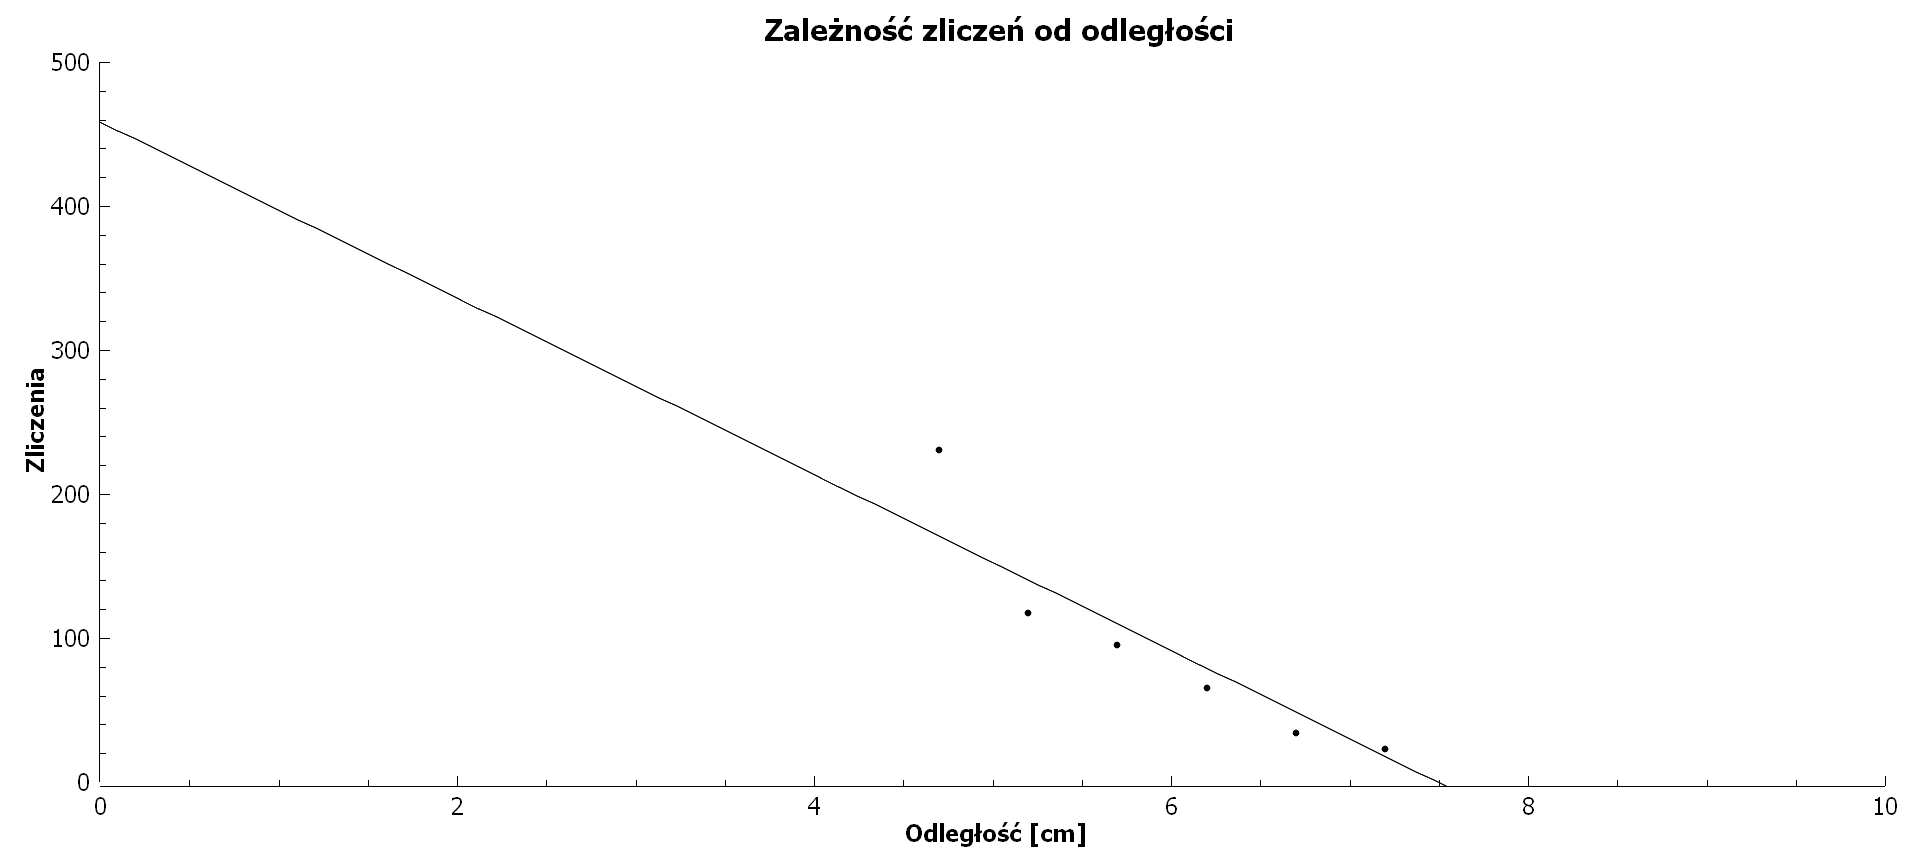
\includegraphics[width=12cm]{wyka} 
\centering
\caption{Punkty pomiarowe wraz z krzywą najlepszego dopasowania}
\label{p2}
\end{figure}

Miejsce zerowe prostej o takich parametrach znajduje się w punkcie $x_{0}=7,49\pm0,38$ cz, przy czym niepewność tego punktu znaleziono stosując Równanie (10) do wzoru $x_{0}=-\hat{b}/\hat{a}$. Aby cząstka dotarła do detektora, to musi pokonać jeszcze warstwę aluminium o grubości 4 $\mu$m, tak więc wartość $x_{0}$ nie jest dokładną wartością zasięgu cząstki w powietrzu. Zasięg $R$ cząstki $\alpha$ wy rażony w mg/cm$^2$ dany jest w tym przypadku wzorem:
\begin{equation}
R=\rho_{p}x_{0}+\rho_{Al} d_{Al},
\end{equation}
gdzie $\rho_{p}, \rho_{Al}$ to kolejno gęstości powietrza i aluminium, a $d_{Al}$ to grubość aluminium \cite{nuc1}. Przyjęto, że $\rho_{p}=1,225$ mg/cm$^3$, a zasięg cząstki w aluminium wyznaczono, korzystając z zależności, że 1 $\mu$m aluminium odpowiada $0,27$ mg/cm$^2$. 
W ten sposób otrzymano wartość $R=10,2586$ mg/cm$^2$. Wyznaczenie niepewności tej wartości jest niemożliwe, gdyż nie są znane niepewności pochodzące od gęstości i grubości powłoki aluminiowej. Taka wartość zasięgu $R$ odpowiada w przybliżeniu energii 7,14 MeV, co stwierdzono, korzystając z tablic zasięgów cząstek \cite{zas}. 
Dodatkowo, dzięki znajomości całkowitego R, można oszacować całkowity zasięg cząstki w powietrzu na $R/\rho_{p}\approx8,37$ cm. 

\begin{center}
\textbf{\subsection*{DYSKUSJA WYNIKÓW I WNIOSKI}}
\end{center}  
Ze względu na błędy pomiarowe ciężko jest wysnuć jakiekolwiek wnioski dotyczące stężenia radonu w powietrzu. Można co najwyżej przyjrzeć się dużej niepewności, jaka narosła wokół stężenia $^{218}$Po. Tak duża niepewność wynika z dużych niepewności względnych związanych z pomiarem zliczeń cząstek $\alpha$. Dodatkowo otrzymane stężenie RaA jest dosyć niskie, wynika to prawdopodobnie z tego, iż miejsce zasysania powietrza znajdowało się w pobliżu drzwi, co narażało je na wietrzenie jak i zostało ono już wcześniej wyeksploatowane. Dodatkowy wpływ wywarła czułość detektora, który nie odbierał tak wielu zliczeń, jak inne detektory z pracowni. Z całą pewnością lepsze wyniki można by było uzyskać, gdyby każdej osobie przysługiwał jej własny odkurzacz jaki własne, dobrze odizolowane miejsce, z którego można pobrać próbkę. Szacowanie energii i zasięgu cząstek zwróciło akceptowalne wyniki, pomimo pośpiechu i małej liczby zliczeń związanej z każdą wysokością. Dodatkowo istnieją podejrzenia, iż zależność $n(d)$ może być zależnością eksponencjalną, jednakże zbyt mała liczba punktów pomiarowych nie pozwala na prawidłową ocenę natury tej zależności.

\begin{center}
\begin{thebibliography}{9}


 \bibitem{m1}
  K.P. Markov, N.W. Rijabov, K.N. Stas, 
  \emph{A rapid method for estimating the radiation hazard associated with the presence of radon daughter products in air},
  Atomnaja Energia 12, 1962, s. 315

 \bibitem{r1}
  R. Nowak,
  \emph{Statystyka dla fizyków},
  PWN, Warszawa, 2002, s. 276.
  
  \bibitem{tay2}
 J. R. Taylor,
 \emph{Wstęp do analizy błędu pomiarowego},
 PWN, Warszawa, 1995, s. 81.
 
  \bibitem{tay4}
 J. R. Taylor,
 \emph{Wstęp do analizy błędu pomiarowego},
 PWN, Warszawa, 1995, s. 169. 
 
 \bibitem{nuc1}
 Michael F. L'Annunziata,
 \emph{Radioactivity: Introduction and History},
 Elsevier, Amsterdam, 2007, s. 81. 
 
 \bibitem{zas}
 L. C. Northcliffe, R. F. Schilling, 
 \emph{RANGE AND STOPPING - POWER TABLES FOR HEAVY IONS},
 Cyclotron Institute, Texas A\&M University, College Station, Texas 1970, s. 233.
 
 \end{thebibliography}
\end{center}

\end{document}